{
Vi viser fejlen i kodeboks \ref{pseudo_udtraek_org}, ved en håndkørsel
på billedet i figur \ref{region_init}, hvor vi traverserer snittet vist
i figur \ref{impUdtraek_kantpunkter}.  Dette horisontale snit ligger
således, at vi rammer alle tre sorte kasser. Vi bevæger os fra venstre
mod højre når vi finder regioner i horisontale snit.

\begin{figure}[!p]
    \setlength\fboxsep{0pt}
    \setlength\fboxrule{0.5pt}
    \centering
    \subfloat[Original]{
        \label{region_init}
        \fbox{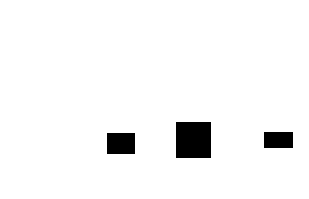
\includegraphics[width=0.4\textwidth]{afsnit/implementation/billeder/billedbehandling/binary_init}}}\hspace{1em}
    \subfloat[1. iteration]{
        \label{region1}
        \fbox{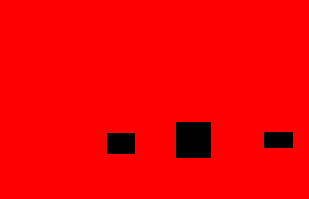
\includegraphics[width=0.4\textwidth]{afsnit/implementation/billeder/billedbehandling/binary_s1}}}\\
    \subfloat[2. iteration]{
        \label{region2}
        \fbox{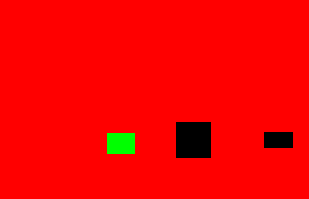
\includegraphics[width=0.4\textwidth]{afsnit/implementation/billeder/billedbehandling/binary_s2}}}\hspace{1em}
    \subfloat[3. iteration]{
        \label{region3}
        \fbox{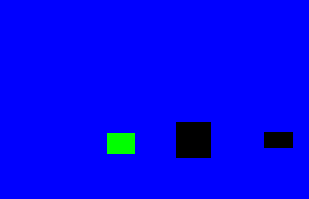
\includegraphics[width=0.4\textwidth]{afsnit/implementation/billeder/billedbehandling/binary_s3}}}\\
    \subfloat[4. iteration]{
        \label{region4}
        \fbox{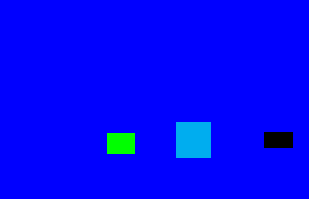
\includegraphics[width=0.4\textwidth]{afsnit/implementation/billeder/billedbehandling/binary_s4}}}\hspace{1em}
    \subfloat[5. iteration]{
        \label{region5}
        \fbox{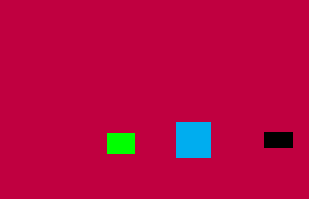
\includegraphics[width=0.4\textwidth]{afsnit/implementation/billeder/billedbehandling/binary_s5}}}\\
    \subfloat[6. iteration]{
        \label{region6}
        \fbox{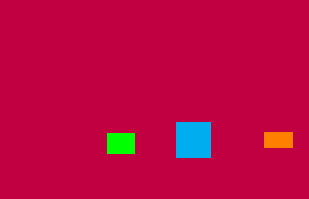
\includegraphics[width=0.4\textwidth]{afsnit/implementation/billeder/billedbehandling/binary_s6}}}\hspace{1em}
    \subfloat[7. iteration]{
        \label{region7}
        \fbox{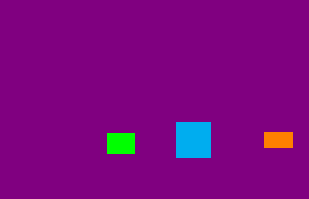
\includegraphics[width=0.4\textwidth]{afsnit/implementation/billeder/billedbehandling/binary_s7}}}
        \caption[]{Iterationerne for kodeboks \ref{pseudo_udtraek_org}
        ved snittet vist i figur \ref{impUdtraek_kantpunkter}}
    \label{region_extract}
\end{figure}
\begin{enumerate}
    \item Linjestykket $Ae_1$ bliver malet rødt. Hele den hvide baggrund
        males rød og denne region returneres.
    \item Linjestykket $e_1e_2$ males. Den første kasse fra venstre
        bliver malet grøn. Denne region returneres.
    \item Linjestykket $e_2e_3$ males blåt, men dette er den samme region som
        fundet i første iteration. Der returneres alligevel en ny
        region.
    \item Linjestykket $e_3e_4$ males lyseblåt og udgøres af den
        midterste kasse, der returneres som en ny region.
    \item Linjestykket $e_4e_5$ bliver malet og endnu engang findes en
        region som vi allerede har fundet.
    \item Linjestykket $e_5e_6$ males orange og vi finder den sidste
        kasse.
    \item Linjestykket $e_6B$ males lilla og vi returnerer igen en
        allerede fundet region.
\end{enumerate}

Vi ender altså med at have returneret syv regioner, ligesom antallet af
segmenter på snittet, men når vi kigger på resultatet, i figur
\ref{region7}, er der kun fire forskellige farver. Vi returnerer den
samme region, baggrunden, som i originalen var hvid, i alt fire gange.
}

% vim: set tw=72 spell spelllang=da:
